\chapter{ToD Simulator}
\label{chap:tod_simulator}
This chapter will elaborate on the ToD simulation framework described in \cite{valeriopaper}, which composes the basis for the work carried out over the course of this thesis.

\section{Network simulator: OMNeT++}    
OMNeT++ is a versatile discrete event simulation framework that has been widely used in the research community, particularly in the field of network simulations. It is based on C++ and provides a modular and extensible architecture that allows users to create complex simulations of communication networks, such as the Internet or wireless networks.

The modular architecture of OMNeT++ enables users to build simulations by using pre-existing components and creating custom ones. This makes it possible to create simulations that are tailored to specific research needs and to easily modify and extend existing simulations. Its support for discrete event simulation, which models the behavior of a system as a series of discrete events, allows for the accurate modeling of network behaviors and for the simulation of large-scale networks.

OMNeT++ provides a feature-rich IDE, shown in \figurename~\ref{fig:omnetpp_interface_tod_network}, and includes built-in support for visualizing simulation results, which are useful for analyzing the behavior of a network and identifying performance bottlenecks. This makes it easier to understand the behavior of complex communication systems and to identify potential areas for improvement~\cite{OmnetVarga2010}.

\begin{figure}[t]
    \centering
    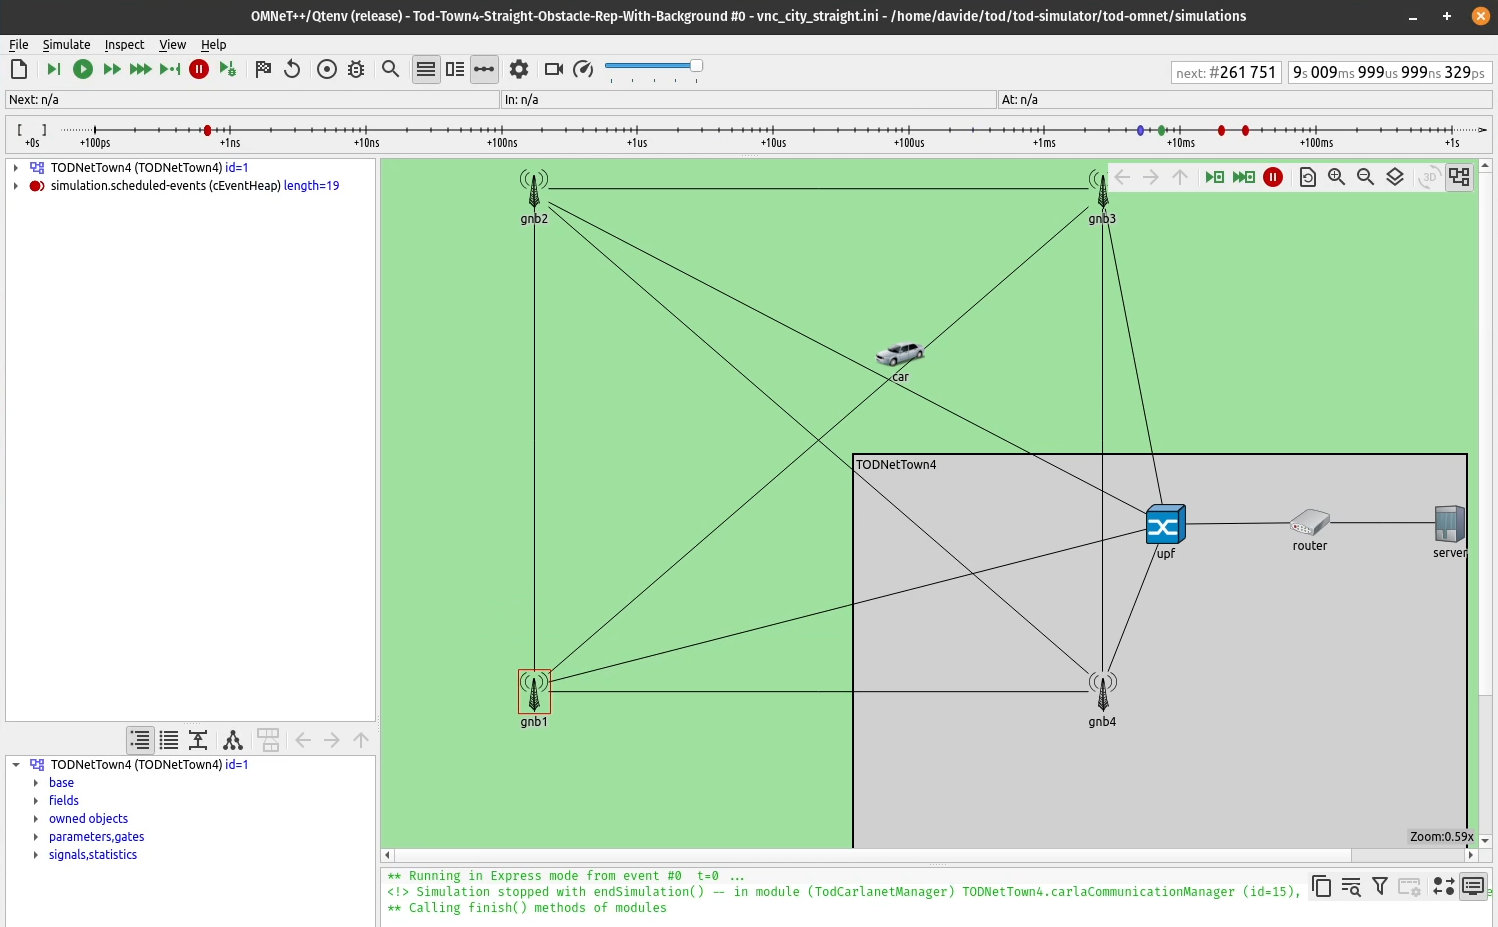
\includegraphics[width=\textwidth]{tod_simulator/omnetpp_interface_tod_network}
    \caption{OMNeT++ GUI (Qtenv) showing the basic network used for simulations}
    \label{fig:omnetpp_interface_tod_network}
\end{figure}

The simulator itself lacks the appropriate modules for TCP/IP and other Internet-related protocols, as well as the ones needed to simulate the 5G radio communications. They are provided by INET and Simu5G.

INET \cite{inetwebsite} is an open-source model library that provides protocols, agents, and other models for simulating communication networks. It contains models for the Internet stack (TCP, UDP, IPv4, IPv6, etc.) and some wireless and wired link layer protocols, such as Ethernet and PPP, among others. It is used as a base for expansion by several other simulation frameworks for the purpose of simulating vehicular networks, overlay and peer-to-peer networks, LTE or 5G.

Simu5G \cite{simu5gwebsite} \cite{9211504} is a 5G New Radio (NR) simulator for the OMNeT++ simulation framework based on the now-deprecated SimuLTE library by the same developers. It incorporates all models from INET and allows researchers to simulate TCP/IP networks including 5G NR interfaces. Simu5G provides models for the data plane of 5G RAN and core networks including the radio links, in both Frequency Division Duplexing and Time Division Duplexing modes, with various types of base stations. It also includes all models from SimuLTE for 4G/LTE networks.




\section{Driving simulator: CARLA}

CARLA (CAR Learning to Act) is an open-source simulator developed from the ground up to support autonomous driving research. It is designed to create a high-fidelity 3D environment that mirrors real-world urban environments, allowing users to test and develop autonomous driving algorithms in a safe, controlled, and cost-effective manner. It leverages Unreal Engine for rendering, which provides high-quality graphics and realistic lighting effects.

The environment provided by CARLA includes city streets, highways, intersections, and various types of roads. It can be customized with different road layouts, buildings, lighting conditions, and weather settings.

In addition, it simulates the behavior of various types of vehicles, including cars, trucks, and buses, with realistic physics and dynamics. This includes accurate modeling of vehicle acceleration, braking, steering, and collision detection. It supports a variety of sensors commonly used in autonomous driving, including cameras, lidars, radars, and GPS.

CARLA provides a Python client API that allows developers to interact with the simulation programmatically. This API enables tasks such as spawning and controlling vehicles, retrieving sensor data, and creating custom scenarios \cite{carla-pmlr-v78-dosovitskiy17a}.

By default, the CARLA server runs the simulation as quickly as it can, in what is called \texttt{asynchronous mode}. The feature that makes it possible for it to work together with OMNeT++ is its \texttt{synchronous mode}.
As the name implies, it allows the server to be kept in sync with the client, and to use all the time it needs to compute each simulation step. This is ideal for slower client applications as well. In the case of the ToD simulation framework, as many components are being simulated in both programs and thus simulated time is much slower than real time on common PC hardware, asynchronous mode would be unusable.



\section{ToD Simulation Framework}
% In order to make the two simulators work together, some sort of intermediary software is required. The Message-Oriented Middleware devised in \cite{valeriopaper} takes care of that, keeping them in constant synchronization.
% It's made up of two components, each one integrated into the respective simulator's API: As a OMNeT++ C++ component and as a CARLA Python client.

% The two simulators use and need different time-steps for their respective duties. In fact, the network simulation performed by OMNeT++ necessitates a much finer time resolution than a vehicle simulation as it has to take care of the whole protocol stack and physical transmission of signals. A proper time orchestrator is needed, in order to avoid incoherent clocks that would lead to unusable simulation results. For this, the OMNeT++ clock is leveraged and the simulator takes on the duty of advancing CARLA's simulation when needed.

%The middleware keeps a mapping of the actors in the CARLA world with the corresponding user equipment in OMNeT++ and updates the locations accordingly, as the movement of vehicles impacts network performance. The distance between a vehicle and its base station via the cellular network affects radio channel quality, and the network simulator must accurately reflect these dynamics to provide an accurate simulation environment.

The ToD simulation framework described in \cite{valeriopaper} is used as the basis for this thesis' experiments and expansion. This section provides a description of its architecture and inner workings.

\subsection{Co-simulation architecture}

In order to make the co-simulation model work, it is firstly essential to clarify the separation of concerns for the two simulators involved - The OMNeT++ network simulator and the CARLA driving simulator - of which the names provide an intuitive description.

OMNeT++ is responsible for simulating the network connection between the HV and the ToD operator, that is, the protocol stack for the UE on the vehicle, the gNodeBs, UPF, and the ToD remote host. It is also in charge of generating the timed events of the application and interacting with the CARLA application components by message passing.

CARLA is responsible for implementing the physical world, including all vehicle dynamics, simulation of sensors and actuators, traffic lights, roads, and pedestrians. It runs the application layer of the ToD driving simulator, including the operator, which is derived from the BehaviorAgent provided by the CARLA library \cite{carladoc}. It is able to calculate a path from the starting point on the map to one or more destinations, following roads and speed limits, and drive the vehicle using the data from its camera and sensor array.

A message-oriented middleware is distributed into two separate components, each integrated into one simulator, which communicate over a network connection. This also allows the two sides to run on separate systems if necessary. They operate in a request-reply model, with requests performed on the OMNeT++ side and replies sent by the CARLA side. \figurename~\ref{fig:tod_sim_architecture} shows a schematic representation of the framework's architecture.

\begin{figure}[h]
    \centering
    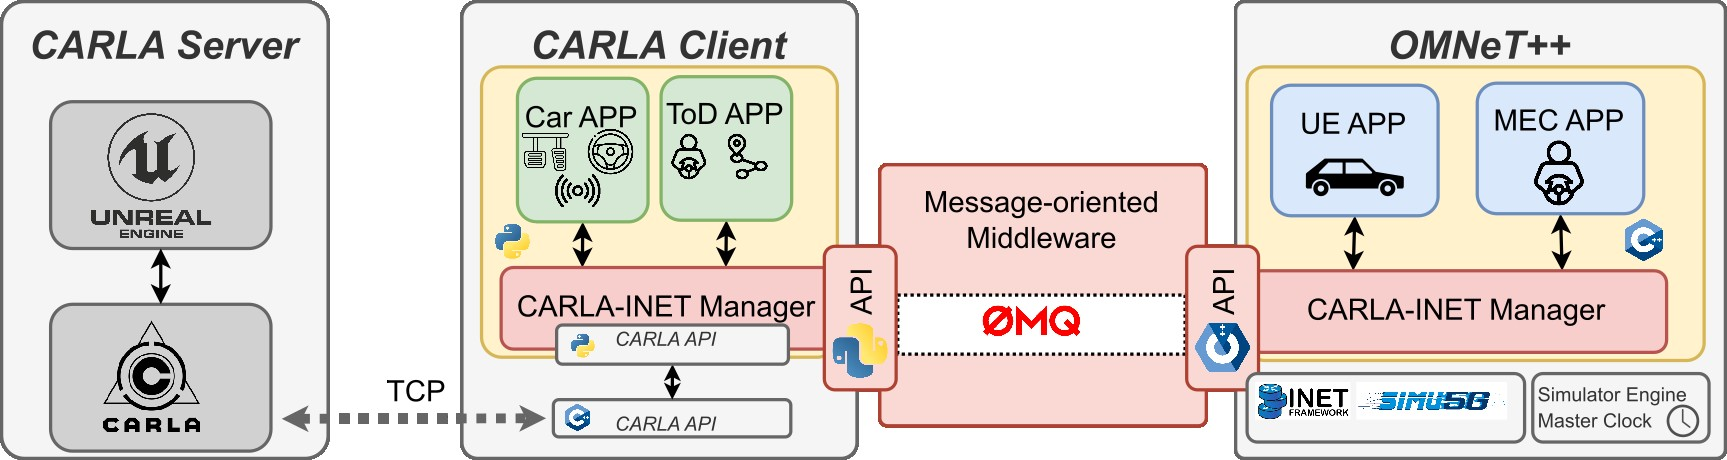
\includegraphics[width=\textwidth]{valeriopaper/tod_sim_architecture.jpg}
    \caption{Architecture of the ToD simulation framework, from \cite{valeriopaper}}
    \label{fig:tod_sim_architecture}
\end{figure}

Each of the two simulators comes with an internal clock, which keeps the simulation time. They also have different needs for its resolution, as the events taking place in the network simulation are much more frequent than those in the driving simulation (picoseconds as opposed to milliseconds). Because of this, the main clock is kept by the component on the OMNeT++ side and it is in charge of sending messages that trigger a world tick to its CARLA correspondent at the required interval.

\subsection{The simulation process}

At the start of each simulation, the OMNeT++ component sends the CARLA component an initialization message containing the required configuration parameters. These include the run ID, random seed, list of nodes, actor IDs and types, and name of the route configuration file. The CARLA component replies with its initial timestamp and the position of each actor that is configured to be synchronized on both sides.

Over the duration of the simulation, the OMNeT++ component schedules a repeating event which sends a message to the CARLA component with the purpose of triggering a simulation step. This message is received by the CARLA side and a simulation step is triggered. A reply is sent back containing each node's position to be updated on the network simulator side.
Different types of messages exist to make the ToD service work, which include the request to generate and send the vehicle sensor data to the operator, the computation of the instructions to send back to the vehicle, and the reply with the controls to be applied. They are simulated as if they were going through the network and are subject to the delay caused by varying network conditions over the vehicle's movement with respect to the base stations.

Within each response sent from CARLA to the OMNeT++ side, the status of the simulation is included, and its purpose is to report whether or not the simulation is due to finish and for which reason, such as a time limit having been reached or a collision having occurred. At that point, the OMNeT++ component sends a finish simulation message, the CARLA simulator terminates its side of the simulation and replies with an acknowledgment, and the network simulator finally terminates its side, marking the end of the whole simulation process.


\subsection{Additions}
In order to carry out some of the scenarios discussed in this thesis, modifications to the aforementioned framework were introduced, the most relevant ones are:
\begin{itemize}
    \item A feature was added so that the route configuration file can contain instructions for where to place an obstacle, which blueprint it uses, which way it faces, and whether it is present in the simulated world from the start of each simulation run or it is spawned when the HV's center point is within a set distance from its configured spawn point (Euclidean distance). A configuration option is also available to specify whether the obstacle vehicle will have CARLA's basic autopilot enabled. Scenarios with this kind of configuration were considered but, due to the agent's limitations, they were not explored further.

    \item A new kind of actor was introduced: the background vehicle, which is used in some of the experiments. The background moving vehicles follow the same implementation as the operator for the HV, but instead of being run through the network they are contained within the CARLA application layer, and ticks at regular intervals are sent to them by the ToD simulator middleware's environment handler. Their operation is thus not affected by any delay and the camera and sensor data are instantly available to the operator at all times. They are linked to background-inducing network nodes in the OMNeT++ simulation so that their location is updated at all times in the simulated network as well.
\end{itemize}

